\chapter{系统设计与架构}
跨界服务将跨越不同行业、组织、价值链等边界的服务进行深度融合和模式创新,为用户提供多维度、高质量、富价值的跨界服务,成为现代服务业发
展的重要创新途径。跨界服务平台是各类跨界服务集成的支撑系统,相比传统的服务集成,跨界服务融合需开展模式、生态、环境、质量、价值等多维深度融合。
为将提出的算法与应用相结合,本文依托于国家重点研发计划专项《现代服务业共性关键技术研发及应用示范》的子课题《跨界服务集成方法与支撑载体》,
在跨界服务平台设计并实现了服务智能调用引擎,本章主要对跨界服务平台和智能调用引擎进行介绍。

\section{跨界服务系统}
本文作者所在的课题组系统性地研究了跨界服务相关理论,并形成了跨界服务原型系统JTangYdrail(图\ref{fig:logo}),
本节主要介绍系统整体架构以及跨界服务系统中两个核心模块服务交换机和服务路由器。
\begin{figure}[htbp]
    \centering
    
\includegraphics[width=6cm]{./images/jianmu.jpg}
    \caption{跨界服务系统 logo}
    \label{fig:logo}
  \end{figure}
  跨界服务系统是针对跨界服务运行时呈现高维异构、复杂动态、开放分布的特点,解决跨界服务网络管理中高效接入、安
  全交换、智能路由等关键技术,形成的跨界服务集成工程化方法,研制软硬件结合的跨
  界服务集成及运行支撑载体,包括跨界服务集成设计软件套件、服务交换机与路由器硬
  件环境。

  海量跨界服务分布于服务网络中,不同服务之间相互操作,通过服务交换及路由技术,实现跨界服务的查找、调用
  及跨界服务间的交互,同时利用基于认证授权的开放服务安全交换技术,保证交换
  过程中的数据安全。服务交换机和服务路由器是支撑载体的关键,采用软硬结合
  的设计方案来实现,如图\ref{fig:system}所示,服务交换机实现跨界服务的高效接入、访问控制、消
  息映射、认证授权等功能,实现域内企业服务的安全可靠的开放,其架构包括设施层(机
  柜、电源、接口等)、设备层(计算服务器、存储服务器)、网络层(虚拟路由器、虚拟
  防火墙)、应用层(服务接入、访问控制、服务缓存等)。服务路由器提供服务聚合、
  服务查找、服务路由等能力,把异构服务联成网络,是跨界服务互联的基础设施,其架
  构包括设施层(机柜、电源、接口等)、设备层(计算服务器、存储服务器)、网络层(状
  态感知、消息路由等功能)、应用层(服务索引、服务查找、服务路由等)。

  \begin{figure}[htbp]
    \centering
    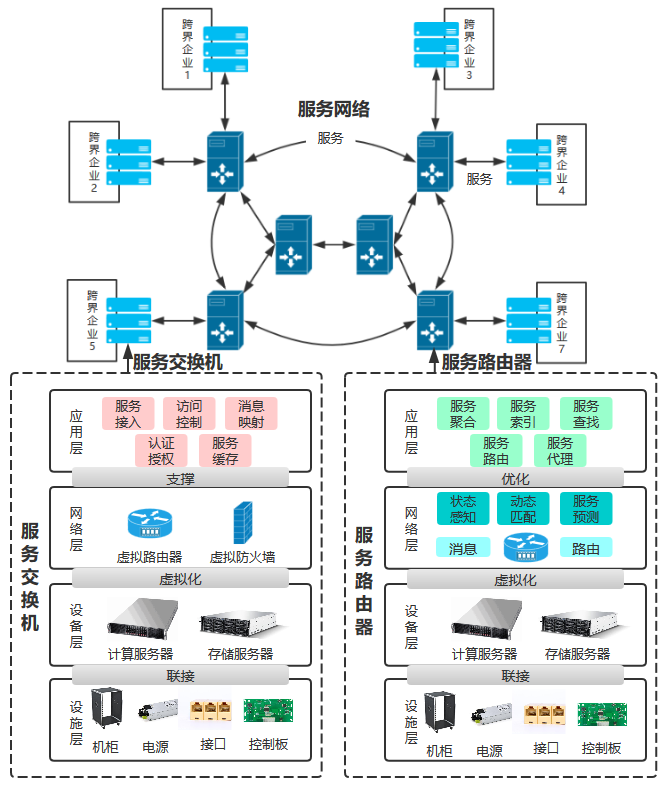
\includegraphics[width=8cm]{./images/system.png}
    \caption{JTangYdrail系统架构}
    \label{fig:system}
  \end{figure}

  服务交换机是跨界服务网络上最下层节点,
  使用服务地址在交换层接收并转发服务相关的数据,与实际服务直接相关,
  是服务的拥有者以及一次服务远程调用的发起者,
如图\ref{fig:switchboard}所示,主要包含以下几个模块:

1)The registry module :维护企业的服务信息和业务数据,
服务成功注册后,服务信息将存储在本地,并且其元数据将通过泛洪或其他方式广播到整个网络。
此后不久,其他服务交换机即可搜索和使用该服务交换机上服务。

2)The adapter module :旨在支持环境异构,AdM提供了各种适配器,可以通过不同的语言实现这些适配器,以实现与异构服务的通信。
在语义上兼容前提下,尽管硬件和软件平台,语言和API不同,但连接到不同适配器的各种服务在跨界服务系统仍将被连接和集成。

3)The policy module:使用多种策略来提高性能,代理策略使用户可以通过代理调用服务,服务交换机的负载平衡策略通过增加进程数来实现可伸缩性和负载平衡,
服务缓存策略使某些节点可以缓存服务调用的结果,从而可以充分利用网络中边缘节点的资源。 

4)The mapping module:旨在为用户带来便利,以特定格式调用服务或接收结果。
 提供了直观的图形界面,供用户生成规则文件。 
 
5)The authentication module:是基于密钥加密技术设计的,并使用基于角色的访问控制策略来保护数据的安全性。

  \begin{figure}[htbp]
    \subfloat[JTangYdrail 服务交换机软件架构]{
      \centering
      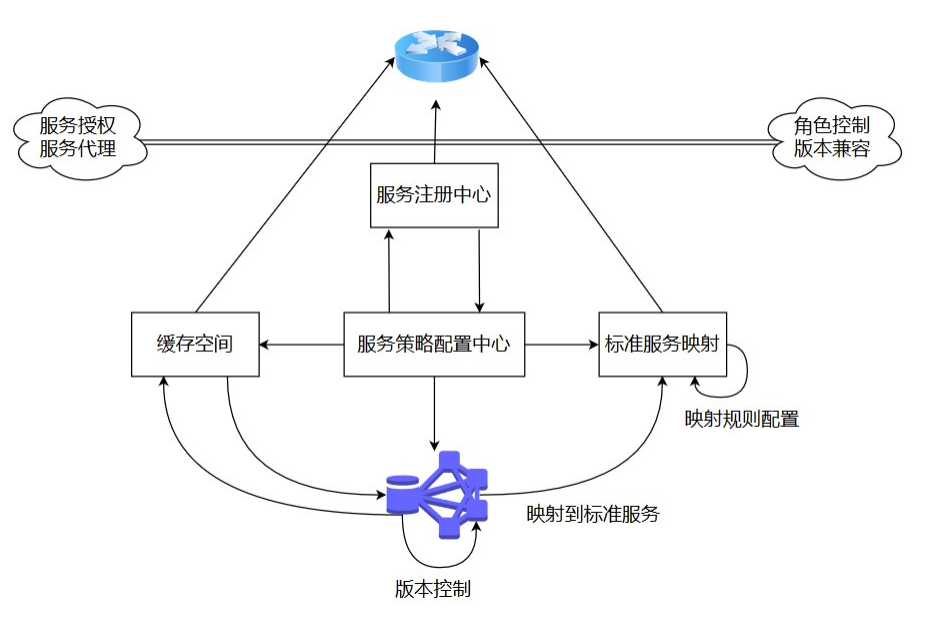
\includegraphics[width=8cm]{./images/switchboard.png}
      \label{fig:switchboard}
    }
    \subfloat[JTangYdrail 服务路由器软件架构]{
      \centering
      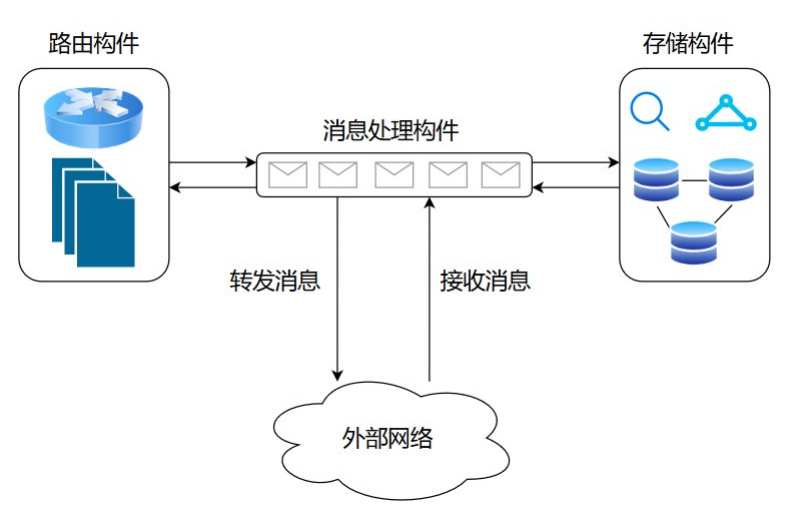
\includegraphics[width=10cm]{./images/router.png}
      \label{fig:router}
    }
    \caption{服务交换机和服务路由器架构}
    \label{fig:loss}
    \end{figure}


    服务路由器是在服务网络中转发服务元信息的网络设备,一方面,服务路由器从服务交换机收集服务信息,并在整个网络中广播数据。 
    另一方面,如果用户调用服务,则服务路由器会将请求转发到相应的服务节点。 
    服务路由器的结构如图\ref{fig:router}所示,其中包含路由组件,存储组件,处理器组件等:

    1)The storage component:由三部分组成:服务缓存,包括一些服务元数据和一些查询结果;
    路由信息,这是整个网络的基础,以及服务网络的结构信息。
    
    2)The routing component:功能是根据服务ID转发服务请求,该服务ID与传统网络中的IP地址完全不同。
    
    3)The processor component:提供内部和外部资源之间的通信机制。消息有两种类型:服务消息和路由消息。
    一旦收到消息,它将由PrC进行预处理,然后传输到路由组件或存储组件。
    
    4)The standardized service component:标准化服务组件设计用于服务网络中功能相似的同类服务,
    当发现Web服务的任何故障时,它可以通过使用标准化服务动态地将服务替换为合适的服务,从而大大提高了服务的可用性和可靠性。


  
  
  \section{服务智能调用引擎}

  \section{系统原型展示}
